% Options for packages loaded elsewhere
\PassOptionsToPackage{unicode}{hyperref}
\PassOptionsToPackage{hyphens}{url}
%
\documentclass[
  12pt,
]{article}
\usepackage{amsmath,amssymb}
\usepackage{iftex}
\ifPDFTeX
  \usepackage[T1]{fontenc}
  \usepackage[utf8]{inputenc}
  \usepackage{textcomp} % provide euro and other symbols
\else % if luatex or xetex
  \usepackage{unicode-math} % this also loads fontspec
  \defaultfontfeatures{Scale=MatchLowercase}
  \defaultfontfeatures[\rmfamily]{Ligatures=TeX,Scale=1}
\fi
\usepackage{lmodern}
\ifPDFTeX\else
  % xetex/luatex font selection
\fi
% Use upquote if available, for straight quotes in verbatim environments
\IfFileExists{upquote.sty}{\usepackage{upquote}}{}
\IfFileExists{microtype.sty}{% use microtype if available
  \usepackage[]{microtype}
  \UseMicrotypeSet[protrusion]{basicmath} % disable protrusion for tt fonts
}{}
\makeatletter
\@ifundefined{KOMAClassName}{% if non-KOMA class
  \IfFileExists{parskip.sty}{%
    \usepackage{parskip}
  }{% else
    \setlength{\parindent}{0pt}
    \setlength{\parskip}{6pt plus 2pt minus 1pt}}
}{% if KOMA class
  \KOMAoptions{parskip=half}}
\makeatother
\usepackage{xcolor}
\usepackage[margin=2.5cm]{geometry}
\usepackage{color}
\usepackage{fancyvrb}
\newcommand{\VerbBar}{|}
\newcommand{\VERB}{\Verb[commandchars=\\\{\}]}
\DefineVerbatimEnvironment{Highlighting}{Verbatim}{commandchars=\\\{\}}
% Add ',fontsize=\small' for more characters per line
\usepackage{framed}
\definecolor{shadecolor}{RGB}{248,248,248}
\newenvironment{Shaded}{\begin{snugshade}}{\end{snugshade}}
\newcommand{\AlertTok}[1]{\textcolor[rgb]{0.94,0.16,0.16}{#1}}
\newcommand{\AnnotationTok}[1]{\textcolor[rgb]{0.56,0.35,0.01}{\textbf{\textit{#1}}}}
\newcommand{\AttributeTok}[1]{\textcolor[rgb]{0.13,0.29,0.53}{#1}}
\newcommand{\BaseNTok}[1]{\textcolor[rgb]{0.00,0.00,0.81}{#1}}
\newcommand{\BuiltInTok}[1]{#1}
\newcommand{\CharTok}[1]{\textcolor[rgb]{0.31,0.60,0.02}{#1}}
\newcommand{\CommentTok}[1]{\textcolor[rgb]{0.56,0.35,0.01}{\textit{#1}}}
\newcommand{\CommentVarTok}[1]{\textcolor[rgb]{0.56,0.35,0.01}{\textbf{\textit{#1}}}}
\newcommand{\ConstantTok}[1]{\textcolor[rgb]{0.56,0.35,0.01}{#1}}
\newcommand{\ControlFlowTok}[1]{\textcolor[rgb]{0.13,0.29,0.53}{\textbf{#1}}}
\newcommand{\DataTypeTok}[1]{\textcolor[rgb]{0.13,0.29,0.53}{#1}}
\newcommand{\DecValTok}[1]{\textcolor[rgb]{0.00,0.00,0.81}{#1}}
\newcommand{\DocumentationTok}[1]{\textcolor[rgb]{0.56,0.35,0.01}{\textbf{\textit{#1}}}}
\newcommand{\ErrorTok}[1]{\textcolor[rgb]{0.64,0.00,0.00}{\textbf{#1}}}
\newcommand{\ExtensionTok}[1]{#1}
\newcommand{\FloatTok}[1]{\textcolor[rgb]{0.00,0.00,0.81}{#1}}
\newcommand{\FunctionTok}[1]{\textcolor[rgb]{0.13,0.29,0.53}{\textbf{#1}}}
\newcommand{\ImportTok}[1]{#1}
\newcommand{\InformationTok}[1]{\textcolor[rgb]{0.56,0.35,0.01}{\textbf{\textit{#1}}}}
\newcommand{\KeywordTok}[1]{\textcolor[rgb]{0.13,0.29,0.53}{\textbf{#1}}}
\newcommand{\NormalTok}[1]{#1}
\newcommand{\OperatorTok}[1]{\textcolor[rgb]{0.81,0.36,0.00}{\textbf{#1}}}
\newcommand{\OtherTok}[1]{\textcolor[rgb]{0.56,0.35,0.01}{#1}}
\newcommand{\PreprocessorTok}[1]{\textcolor[rgb]{0.56,0.35,0.01}{\textit{#1}}}
\newcommand{\RegionMarkerTok}[1]{#1}
\newcommand{\SpecialCharTok}[1]{\textcolor[rgb]{0.81,0.36,0.00}{\textbf{#1}}}
\newcommand{\SpecialStringTok}[1]{\textcolor[rgb]{0.31,0.60,0.02}{#1}}
\newcommand{\StringTok}[1]{\textcolor[rgb]{0.31,0.60,0.02}{#1}}
\newcommand{\VariableTok}[1]{\textcolor[rgb]{0.00,0.00,0.00}{#1}}
\newcommand{\VerbatimStringTok}[1]{\textcolor[rgb]{0.31,0.60,0.02}{#1}}
\newcommand{\WarningTok}[1]{\textcolor[rgb]{0.56,0.35,0.01}{\textbf{\textit{#1}}}}
\usepackage{graphicx}
\makeatletter
\def\maxwidth{\ifdim\Gin@nat@width>\linewidth\linewidth\else\Gin@nat@width\fi}
\def\maxheight{\ifdim\Gin@nat@height>\textheight\textheight\else\Gin@nat@height\fi}
\makeatother
% Scale images if necessary, so that they will not overflow the page
% margins by default, and it is still possible to overwrite the defaults
% using explicit options in \includegraphics[width, height, ...]{}
\setkeys{Gin}{width=\maxwidth,height=\maxheight,keepaspectratio}
% Set default figure placement to htbp
\makeatletter
\def\fps@figure{htbp}
\makeatother
\setlength{\emergencystretch}{3em} % prevent overfull lines
\providecommand{\tightlist}{%
  \setlength{\itemsep}{0pt}\setlength{\parskip}{0pt}}
\setcounter{secnumdepth}{-\maxdimen} % remove section numbering
\usepackage{graphicx}
\usepackage{amsmath}
\usepackage{booktabs}
\usepackage{caption}
\usepackage{fancyhdr}
\usepackage{ragged2e}
\justifying
\pagestyle{fancy}
\fancyhead[L]{Clara Delandre, Majandra Garcia, Paola Biocchi, Coline Leteurte}
\fancyfoot[C]{\thepage}
\usepackage{booktabs}
\usepackage{longtable}
\usepackage{array}
\usepackage{multirow}
\usepackage{wrapfig}
\usepackage{float}
\usepackage{colortbl}
\usepackage{pdflscape}
\usepackage{tabu}
\usepackage{threeparttable}
\usepackage{threeparttablex}
\usepackage[normalem]{ulem}
\usepackage{makecell}
\usepackage{xcolor}
\ifLuaTeX
  \usepackage{selnolig}  % disable illegal ligatures
\fi
\usepackage{bookmark}
\IfFileExists{xurl.sty}{\usepackage{xurl}}{} % add URL line breaks if available
\urlstyle{same}
\hypersetup{
  pdftitle={Predicting Mortgage Yield using Regression Analysis},
  pdfauthor={Group 42},
  hidelinks,
  pdfcreator={LaTeX via pandoc}}

\title{Predicting Mortgage Yield using Regression Analysis}
\author{Group 42}
\date{2025-03-25}

\begin{document}
\maketitle

\section{Introduction}\label{introduction}

The study of A. H. Schaaf, 1966, ``Regional Differences in Mortgage
Financing Costs'' investigates the existence and causes of regional
differences in mortgage financing costs in the United States. These
differences in mortgage yields have decreased in the early 20th century,
however they remained stable after World War 2. The paper explores two
main explanations for this phenomenon:\\
\strut \\
\textbf{1.} differences in investment value due to risk, terms, and
liquidity\\
\textbf{2.} market imperfections such as legal barriers and information
gaps.\\
\strut \\
The data used in this study comes from the Federal Home Loan Bank Board,
which contains interest rates and fees in 18 SMSAs (Standard
Metropolitan Statistical Areas). The findings suggest that distance from
major financial centers, risk levels, and local demand for savings
significantly affect mortgage yields. However, market structure and
overall savings levels play a lesser role.\\
\strut \\
The aim of this report is to analyze the data and develop a predictive
model to predict Mortgage Yield (\texttt{mortYld}) based on 8
explanatory variables:\\
\strut \\
- \textbf{smsa:} Standard Metropolitan Statistical Areas (18) → Name of
the city/region.\\
- \textbf{mortYld:} Mortgage Yield, in \% → The percentage return on a
mortgage.\\
- \textbf{X1:} Loan-to-Mortgage Ratio, in \% → High values indicate low
down payments.\\
- \textbf{X2:} Distance from Boston, in miles → Measures regional
proximity to financial centers.\\
- \textbf{X3:} Savings per new unit built, in \$ → Indicator of regional
credit demand.\\
- \textbf{X4:} Savings per capita, in \$ → Measures local savings levels
(credit supply).\\
- \textbf{X5:} Population increase, 1950-1960, in \% → Proxy for housing
demand growth.\\
- \textbf{X6:} Percentage of first mortgages from inter-regional banks,
in \% → Indicator of external financing reliance.\\

\begin{center}\rule{0.5\linewidth}{0.5pt}\end{center}

\section{Exploratory Data Analysis
(EDA)}\label{exploratory-data-analysis-eda}

\subsection{Load Data and Libraries}\label{load-data-and-libraries}

\begin{Shaded}
\begin{Highlighting}[]
\CommentTok{\# Load necessary libraries}
\FunctionTok{library}\NormalTok{(ggplot2)}
\end{Highlighting}
\end{Shaded}

\begin{verbatim}
## Warning: le package 'ggplot2' a été compilé avec la version R 4.4.3
\end{verbatim}

\begin{Shaded}
\begin{Highlighting}[]
\FunctionTok{library}\NormalTok{(tidyverse)}
\end{Highlighting}
\end{Shaded}

\begin{verbatim}
## Warning: le package 'tidyverse' a été compilé avec la version R 4.4.3
\end{verbatim}

\begin{verbatim}
## Warning: le package 'tibble' a été compilé avec la version R 4.4.3
\end{verbatim}

\begin{verbatim}
## Warning: le package 'tidyr' a été compilé avec la version R 4.4.3
\end{verbatim}

\begin{verbatim}
## Warning: le package 'readr' a été compilé avec la version R 4.4.3
\end{verbatim}

\begin{verbatim}
## Warning: le package 'purrr' a été compilé avec la version R 4.4.3
\end{verbatim}

\begin{verbatim}
## Warning: le package 'dplyr' a été compilé avec la version R 4.4.3
\end{verbatim}

\begin{verbatim}
## Warning: le package 'stringr' a été compilé avec la version R 4.4.3
\end{verbatim}

\begin{verbatim}
## Warning: le package 'forcats' a été compilé avec la version R 4.4.3
\end{verbatim}

\begin{verbatim}
## Warning: le package 'lubridate' a été compilé avec la version R 4.4.3
\end{verbatim}

\begin{verbatim}
## -- Attaching core tidyverse packages ------------------------ tidyverse 2.0.0 --
## v dplyr     1.1.4     v readr     2.1.5
## v forcats   1.0.0     v stringr   1.5.1
## v lubridate 1.9.4     v tibble    3.2.1
## v purrr     1.0.4     v tidyr     1.3.1
## -- Conflicts ------------------------------------------ tidyverse_conflicts() --
## x dplyr::filter() masks stats::filter()
## x dplyr::lag()    masks stats::lag()
## i Use the conflicted package (<http://conflicted.r-lib.org/>) to force all conflicts to become errors
\end{verbatim}

\begin{Shaded}
\begin{Highlighting}[]
\FunctionTok{library}\NormalTok{(dplyr)}
\FunctionTok{library}\NormalTok{(knitr)}
\end{Highlighting}
\end{Shaded}

\begin{verbatim}
## Warning: le package 'knitr' a été compilé avec la version R 4.4.3
\end{verbatim}

\begin{Shaded}
\begin{Highlighting}[]
\FunctionTok{library}\NormalTok{(kableExtra)}
\end{Highlighting}
\end{Shaded}

\begin{verbatim}
## Warning: le package 'kableExtra' a été compilé avec la version R 4.4.3
\end{verbatim}

\begin{verbatim}
## 
## Attachement du package : 'kableExtra'
## 
## L'objet suivant est masqué depuis 'package:dplyr':
## 
##     group_rows
\end{verbatim}

\begin{Shaded}
\begin{Highlighting}[]
\FunctionTok{library}\NormalTok{(xtable)}
\end{Highlighting}
\end{Shaded}

\begin{verbatim}
## Warning: le package 'xtable' a été compilé avec la version R 4.4.3
\end{verbatim}

\begin{Shaded}
\begin{Highlighting}[]
\FunctionTok{library}\NormalTok{(MASS)}
\end{Highlighting}
\end{Shaded}

\begin{verbatim}
## 
## Attachement du package : 'MASS'
## 
## L'objet suivant est masqué depuis 'package:dplyr':
## 
##     select
\end{verbatim}

\begin{Shaded}
\begin{Highlighting}[]
\FunctionTok{library}\NormalTok{(car)}
\end{Highlighting}
\end{Shaded}

\begin{verbatim}
## Warning: le package 'car' a été compilé avec la version R 4.4.3
\end{verbatim}

\begin{verbatim}
## Le chargement a nécessité le package : carData
\end{verbatim}

\begin{verbatim}
## Warning: le package 'carData' a été compilé avec la version R 4.4.3
\end{verbatim}

\begin{verbatim}
## 
## Attachement du package : 'car'
## 
## L'objet suivant est masqué depuis 'package:dplyr':
## 
##     recode
## 
## L'objet suivant est masqué depuis 'package:purrr':
## 
##     some
\end{verbatim}

\begin{Shaded}
\begin{Highlighting}[]
\FunctionTok{library}\NormalTok{(magrittr)}
\end{Highlighting}
\end{Shaded}

\begin{verbatim}
## Warning: le package 'magrittr' a été compilé avec la version R 4.4.3
\end{verbatim}

\begin{verbatim}
## 
## Attachement du package : 'magrittr'
## 
## L'objet suivant est masqué depuis 'package:purrr':
## 
##     set_names
## 
## L'objet suivant est masqué depuis 'package:tidyr':
## 
##     extract
\end{verbatim}

\begin{Shaded}
\begin{Highlighting}[]
\CommentTok{\# Read data}
\NormalTok{df }\OtherTok{\textless{}{-}} \FunctionTok{read.csv}\NormalTok{(}\StringTok{"myield.csv"}\NormalTok{)}

\CommentTok{\# Rename columns for easier reference}
\FunctionTok{colnames}\NormalTok{(df) }\OtherTok{\textless{}{-}} \FunctionTok{c}\NormalTok{(}\StringTok{"smsa"}\NormalTok{, }\StringTok{"mortYld"}\NormalTok{, }\StringTok{"X1"}\NormalTok{, }\StringTok{"X2"}\NormalTok{, }\StringTok{"X3"}\NormalTok{, }\StringTok{"X4"}\NormalTok{, }\StringTok{"X5"}\NormalTok{, }\StringTok{"X6"}\NormalTok{)}

\CommentTok{\# Display first few rows}
\FunctionTok{kable}\NormalTok{(}\FunctionTok{head}\NormalTok{(df), }\AttributeTok{caption =} \StringTok{"First few rows of the dataset"}\NormalTok{) }\SpecialCharTok{\%\textgreater{}\%} \FunctionTok{kable\_styling}\NormalTok{()}
\end{Highlighting}
\end{Shaded}

\begin{longtable}[t]{lrrrrrrr}
\caption{\label{tab:unnamed-chunk-1}First few rows of the dataset}\\
\toprule
smsa & mortYld & X1 & X2 & X3 & X4 & X5 & X6\\
\midrule
Los Angeles-Long Bea & 6.17 & 78.1 & 3042 & 91.3 & 1738.1 & 45.5 & 33.1\\
Denver & 6.06 & 77.0 & 1997 & 84.1 & 1110.4 & 51.8 & 21.9\\
San Francisco-Oaklan & 6.04 & 75.7 & 3162 & 129.3 & 1738.1 & 24.0 & 46.0\\
Dallas-Fort Worth & 6.04 & 77.4 & 1821 & 41.2 & 778.4 & 45.7 & 51.3\\
Miami & 6.02 & 77.4 & 1542 & 119.1 & 1136.7 & 88.9 & 18.7\\
\addlinespace
Atlanta & 6.02 & 73.6 & 1074 & 32.3 & 582.9 & 39.9 & 26.6\\
\bottomrule
\end{longtable}

\begin{Shaded}
\begin{Highlighting}[]
\CommentTok{\# Count missing values}
\FunctionTok{colSums}\NormalTok{(}\FunctionTok{is.na}\NormalTok{(df))}
\end{Highlighting}
\end{Shaded}

\begin{verbatim}
##    smsa mortYld      X1      X2      X3      X4      X5      X6 
##       0       0       0       0       0       0       0       0
\end{verbatim}

Here is a display of the data, on the first few rows of the dataset. It
contains mortgage yield (mortYld) as the dependent variable and six
variables (X1 to X6). smsa represents the Standard Metropolitan
Statistical Area which is the name of the city/region. We can observe
that all data are numerical values and there is no missing value for
each region.

\subsection{Univariate Analysis}\label{univariate-analysis}

\subsubsection{Summary Statistics}\label{summary-statistics}

\begin{Shaded}
\begin{Highlighting}[]
\CommentTok{\# Summary Statistics}
\NormalTok{summary\_stats }\OtherTok{\textless{}{-}} \FunctionTok{summary}\NormalTok{(df[, }\FunctionTok{colnames}\NormalTok{(df) }\SpecialCharTok{!=} \StringTok{"smsa"}\NormalTok{])}
\FunctionTok{kable}\NormalTok{(summary\_stats, }\AttributeTok{caption =} \StringTok{"Summary Statistics of Variables"}\NormalTok{) }\SpecialCharTok{\%\textgreater{}\%} \FunctionTok{kable\_styling}\NormalTok{()}
\end{Highlighting}
\end{Shaded}

\begin{longtable}[t]{llllllll}
\caption{\label{tab:unnamed-chunk-3}Summary Statistics of Variables}\\
\toprule
 & mortYld & X1 & X2 & X3 & X4 & X5 & X6\\
\midrule
 & Min.   :5.280 & Min.   :67.00 & Min.   :   0 & Min.   : 32.3 & Min.   : 582.9 & Min.   : 7.50 & Min.   : 2.00\\
 & 1st Qu.:5.678 & 1st Qu.:70.03 & 1st Qu.: 648 & 1st Qu.: 85.9 & 1st Qu.: 792.9 & 1st Qu.:23.18 & 1st Qu.: 9.55\\
 & Median :5.880 & Median :73.25 & Median :1364 & Median :122.2 & Median :1161.3 & Median :27.35 & Median :18.70\\
 & Mean   :5.841 & Mean   :73.38 & Mean   :1389 & Mean   :159.8 & Mean   :1245.9 & Mean   :33.03 & Mean   :20.95\\
 & 3rd Qu.:6.020 & 3rd Qu.:77.22 & 3rd Qu.:1847 & 3rd Qu.:218.2 & 3rd Qu.:1556.6 & 3rd Qu.:44.10 & 3rd Qu.:30.43\\
\addlinespace
 & Max.   :6.170 & Max.   :78.10 & Max.   :3162 & Max.   :428.2 & Max.   :2582.4 & Max.   :88.90 & Max.   :51.30\\
\bottomrule
\end{longtable}

We can observe that each variable 18 observations corresponding to 18
different SMSAs. Through this summary, we can already observe mortgage
yields don't vary much across regions. Most values are between 5.5\% and
6.2\%, suggesting relatively stable mortgage rates.

Loan-to-mortgage ratios (X1) are concentrated in between 70\% and 78\%,
with low variance. Savings per New Unit Built (X3) are characterized by
a mean bigger than the median, representing a right-skewed distribution
and then large disparities in housing affordability across regions.

-\textgreater{} to complete

\subsubsection{Graphical Representation}\label{graphical-representation}

\begin{Shaded}
\begin{Highlighting}[]
\CommentTok{\# Histogram of Mortgage Yield}
\FunctionTok{ggplot}\NormalTok{(df, }\FunctionTok{aes}\NormalTok{(}\AttributeTok{x =}\NormalTok{ mortYld)) }\SpecialCharTok{+} 
  \FunctionTok{geom\_histogram}\NormalTok{(}\AttributeTok{binwidth =} \FloatTok{0.2}\NormalTok{, }\AttributeTok{fill =} \StringTok{"blue"}\NormalTok{, }\AttributeTok{alpha =} \FloatTok{0.6}\NormalTok{) }\SpecialCharTok{+}
  \FunctionTok{labs}\NormalTok{(}\AttributeTok{title =} \StringTok{"Distribution of Mortgage Yield"}\NormalTok{, }\AttributeTok{x =} \StringTok{"Mortgage Yield (\%)"}\NormalTok{, }\AttributeTok{y =} \StringTok{"Count"}\NormalTok{)}
\end{Highlighting}
\end{Shaded}

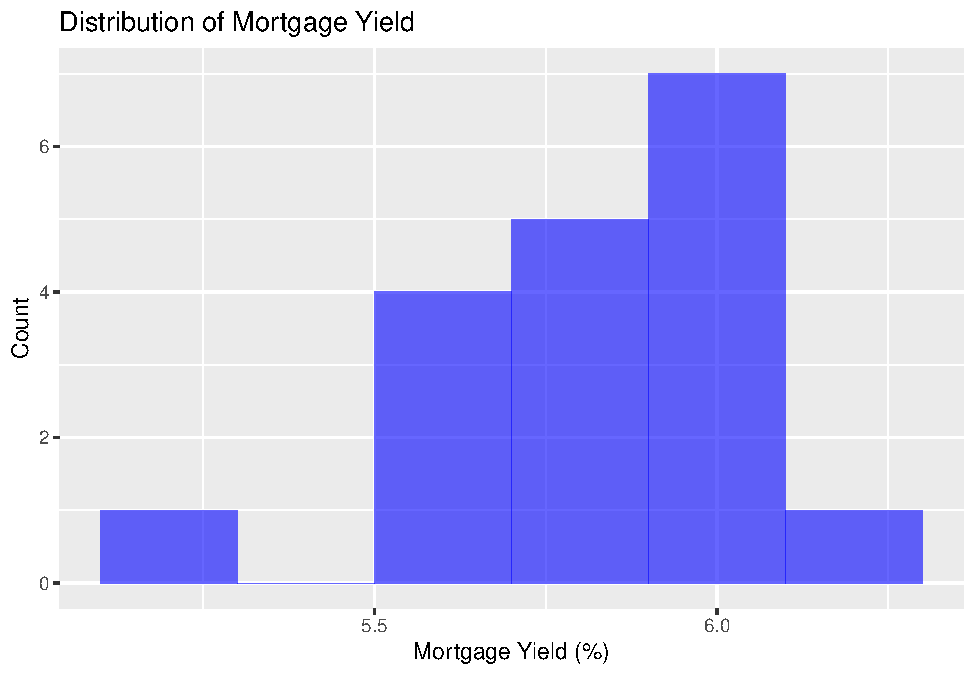
\includegraphics{report1_r1_files/figure-latex/unnamed-chunk-4-1.pdf}

\begin{Shaded}
\begin{Highlighting}[]
\CommentTok{\# Create a named vector where mortgage yield values are associated with their respective SMSAs}
\NormalTok{df }\OtherTok{\textless{}{-}}\NormalTok{ df }\SpecialCharTok{\%\textgreater{}\%} \FunctionTok{arrange}\NormalTok{(}\FunctionTok{desc}\NormalTok{(mortYld))  }

\CommentTok{\# Create a better bar chart}
\FunctionTok{ggplot}\NormalTok{(df, }\FunctionTok{aes}\NormalTok{(}\AttributeTok{x =} \FunctionTok{reorder}\NormalTok{(smsa, mortYld), }\AttributeTok{y =}\NormalTok{ mortYld)) }\SpecialCharTok{+} 
  \FunctionTok{geom\_bar}\NormalTok{(}\AttributeTok{stat =} \StringTok{"identity"}\NormalTok{, }\AttributeTok{fill =} \StringTok{"blue"}\NormalTok{) }\SpecialCharTok{+}
  \FunctionTok{coord\_flip}\NormalTok{() }\SpecialCharTok{+}  \CommentTok{\# Flip coordinates to make labels readable}
  \FunctionTok{labs}\NormalTok{(}\AttributeTok{title =} \StringTok{"Mortgage Yield by SMSA"}\NormalTok{, }\AttributeTok{x =} \StringTok{"SMSA (City)"}\NormalTok{, }\AttributeTok{y =} \StringTok{"Mortgage Yield (\%)"}\NormalTok{) }\SpecialCharTok{+}
  \FunctionTok{theme\_minimal}\NormalTok{()}
\end{Highlighting}
\end{Shaded}

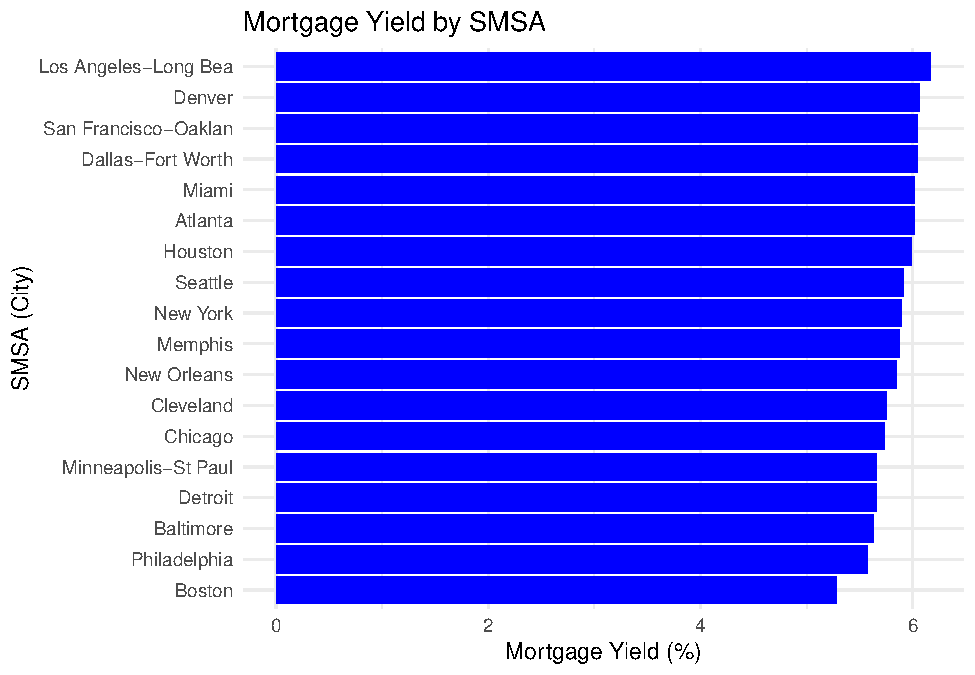
\includegraphics{report1_r1_files/figure-latex/unnamed-chunk-4-2.pdf}

\begin{Shaded}
\begin{Highlighting}[]
\CommentTok{\# Set up a 2x3 grid for multiple histograms}
\FunctionTok{par}\NormalTok{(}\AttributeTok{mfrow =} \FunctionTok{c}\NormalTok{(}\DecValTok{2}\NormalTok{, }\DecValTok{3}\NormalTok{))}

\CommentTok{\# Define variable names}
\NormalTok{var\_names }\OtherTok{\textless{}{-}} \FunctionTok{c}\NormalTok{(}\StringTok{"Loan{-}to{-}Mortgage Ratio"}\NormalTok{, }\StringTok{"Distance from Boston"}\NormalTok{, }
               \StringTok{"Savings per New Unit Built"}\NormalTok{, }\StringTok{"Savings per Capita"}\NormalTok{, }
               \StringTok{"Population Increase"}\NormalTok{, }\StringTok{"First Mortgage from Inter{-}Regional Banks"}\NormalTok{)}

\CommentTok{\# Define colors for better visualization}
\NormalTok{hist\_colors }\OtherTok{\textless{}{-}} \FunctionTok{c}\NormalTok{(}\StringTok{"red"}\NormalTok{, }\StringTok{"blue"}\NormalTok{, }\StringTok{"green"}\NormalTok{, }\StringTok{"purple"}\NormalTok{, }\StringTok{"orange"}\NormalTok{, }\StringTok{"cyan"}\NormalTok{)}

\CommentTok{\# Loop through each variable (X1 to X6) and create a histogram}
\ControlFlowTok{for}\NormalTok{ (i }\ControlFlowTok{in} \DecValTok{1}\SpecialCharTok{:}\DecValTok{6}\NormalTok{) \{}
  \FunctionTok{hist}\NormalTok{(df[[}\FunctionTok{paste0}\NormalTok{(}\StringTok{"X"}\NormalTok{, i)]], }
       \AttributeTok{main =} \FunctionTok{paste}\NormalTok{(}\StringTok{"Histogram of"}\NormalTok{, var\_names[i]),}
       \AttributeTok{xlab =}\NormalTok{ var\_names[i], }
       \AttributeTok{col =}\NormalTok{ hist\_colors[i], }
       \AttributeTok{border =} \StringTok{"black"}\NormalTok{)}
\NormalTok{\}}
\end{Highlighting}
\end{Shaded}

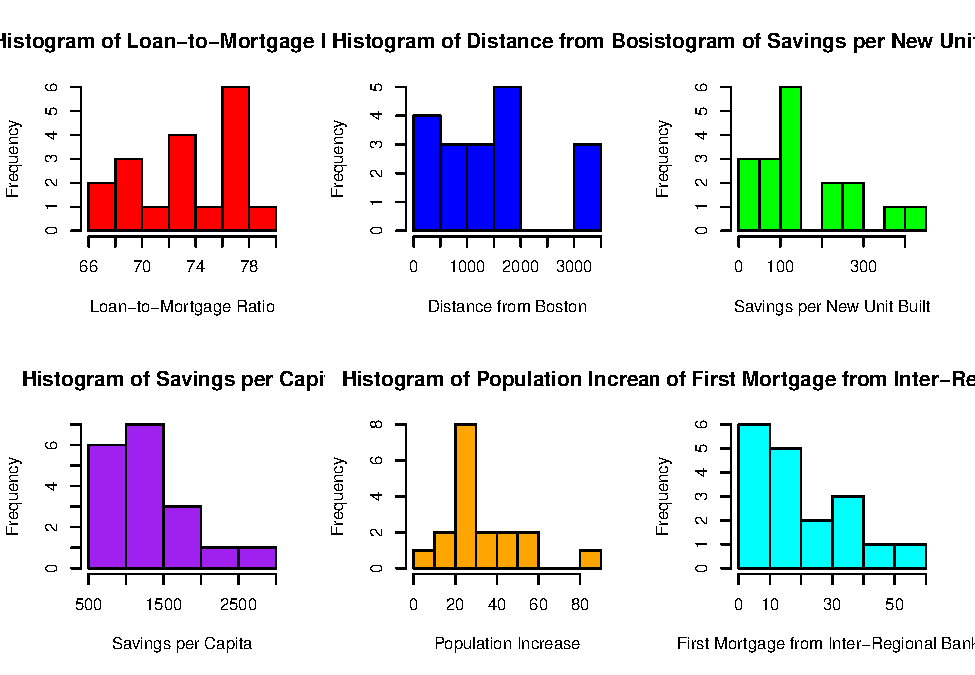
\includegraphics{report1_r1_files/figure-latex/unnamed-chunk-4-3.pdf}

\begin{Shaded}
\begin{Highlighting}[]
\CommentTok{\# Reset plotting parameters to default}
\FunctionTok{par}\NormalTok{(}\AttributeTok{mfrow =} \FunctionTok{c}\NormalTok{(}\DecValTok{1}\NormalTok{, }\DecValTok{1}\NormalTok{))}
\end{Highlighting}
\end{Shaded}

1st graph : doesn't seem to follows a normal distribution.

2nd graph : There is not a huge variation in mortgage yield across
SMSAs, as most bars are at similar heightsbut if we focus on 4 and 6\%,
we see regional differences exist in mortgage yields, possibly due to
economic factors like savings, loan terms, and regional banking
practices.

3rd graph :

The histograms reveal the characteristics of the predictor variables.

The loan-to-mortgage ratio (X1) shows low variance with most values
concentrated between 70\% and 78\%, indicating limited variability
across regions. It might suggest that this variable has limited
predictive power in explaining mortgage yield variation.

Distance from Boston (X2) displays a wide and multimodal distribution,
reflecting substantial geographic spread among SMSAs.

Savings per new unit built (X3) and savings per capita (X4) both exhibit
right-skewed distributions, suggesting that a few cities have notably
higher savings levels.

Population increase (X5) is highly skewed with one major outlier,
indicating that most cities had moderate growth, while a few experienced
rapid expansion. We can also observe potential outliers.

Finally, the percentage of first mortgages from inter-regional banks
(X6) is also right-skewed, with most cities relying minimally on
external financing and a few showing heavy dependence.

These patterns suggest that certain variables may benefit from
transformation prior to regression modeling.

\subsection{Bivariate Numerical
Analysis}\label{bivariate-numerical-analysis}

\subsubsection{Association Analysis}\label{association-analysis}

\begin{Shaded}
\begin{Highlighting}[]
\CommentTok{\# Adjust the plotting window size to be square{-}like (you may need to resize RStudio plot panel)}
\FunctionTok{par}\NormalTok{(}\AttributeTok{mfrow =} \FunctionTok{c}\NormalTok{(}\DecValTok{1}\NormalTok{, }\DecValTok{1}\NormalTok{))  }\CommentTok{\# Reset to 1x1 layout}
\FunctionTok{par}\NormalTok{(}\AttributeTok{mai =} \FunctionTok{c}\NormalTok{(}\DecValTok{1}\NormalTok{, }\DecValTok{1}\NormalTok{, }\DecValTok{1}\NormalTok{, }\DecValTok{1}\NormalTok{))  }\CommentTok{\# Adjust margins to give more space around the plot}
\FunctionTok{par}\NormalTok{(}\AttributeTok{pin =} \FunctionTok{c}\NormalTok{(}\DecValTok{10}\NormalTok{, }\DecValTok{10}\NormalTok{))  }\CommentTok{\# Set plot aspect ratio manually (width and height in inches)}

\CommentTok{\# Select relevant numerical variables}
\NormalTok{selected\_vars }\OtherTok{\textless{}{-}}\NormalTok{ df[, }\FunctionTok{c}\NormalTok{(}\StringTok{"mortYld"}\NormalTok{, }\StringTok{"X1"}\NormalTok{, }\StringTok{"X2"}\NormalTok{, }\StringTok{"X3"}\NormalTok{, }\StringTok{"X4"}\NormalTok{, }\StringTok{"X5"}\NormalTok{, }\StringTok{"X6"}\NormalTok{)]}

\CommentTok{\# Create the scatter plot matrix}
\FunctionTok{pairs}\NormalTok{(selected\_vars, }
      \AttributeTok{main =} \StringTok{"Association Matrix of Variables and mortYld"}\NormalTok{,}
      \AttributeTok{col =} \StringTok{"blue"}\NormalTok{,   }\CommentTok{\# Set color for points}
      \AttributeTok{pch =} \DecValTok{19}\NormalTok{)       }\CommentTok{\# Use solid dots for points}
\end{Highlighting}
\end{Shaded}

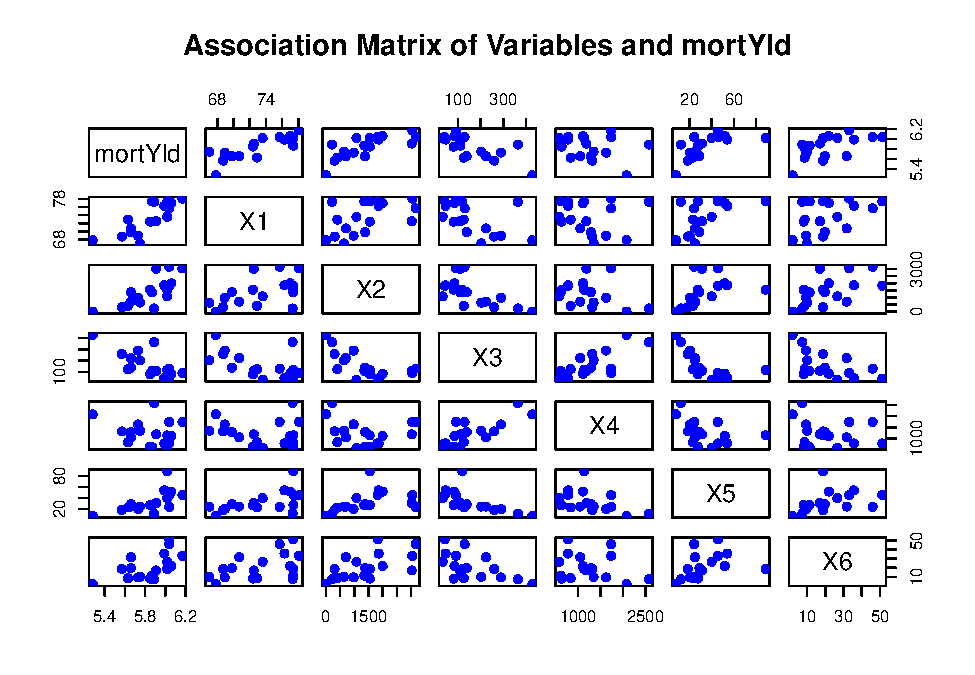
\includegraphics{report1_r1_files/figure-latex/unnamed-chunk-5-1.pdf}

The scatterplot matrix provides a quick visual assessment of linearity,
strength of associations, potential collinearity among predictors, and
outlier detection. It complements numerical analyses like the
correlation matrix and VIF.

We can visualizes bivariate relationships, \textbf{how each variable
relates to the others}, especially to mortYld and assess if a
relationship is linear, curved, or weak, positive or negative.We can
also spot \textbf{outliers} or cities that don't follow the general
trend.

Tell about positive, negative associations, weak, strong ? (week 2 slide
5)

\begin{Shaded}
\begin{Highlighting}[]
\CommentTok{\# Set up a 2x3 grid for multiple scatter plots}
\FunctionTok{par}\NormalTok{(}\AttributeTok{mfrow =} \FunctionTok{c}\NormalTok{(}\DecValTok{2}\NormalTok{, }\DecValTok{3}\NormalTok{))}

\CommentTok{\# Define variable names}
\NormalTok{var\_names }\OtherTok{\textless{}{-}} \FunctionTok{c}\NormalTok{(}\StringTok{"Loan{-}to{-}Mortgage Ratio"}\NormalTok{, }\StringTok{"Distance from Boston"}\NormalTok{, }
               \StringTok{"Savings per New Unit Built"}\NormalTok{, }\StringTok{"Savings per Capita"}\NormalTok{, }
               \StringTok{"Population Increase"}\NormalTok{, }\StringTok{"First Mortgage from Inter{-}Regional Banks"}\NormalTok{)}

\CommentTok{\# Define colors for better visualization}
\NormalTok{point\_colors }\OtherTok{\textless{}{-}} \FunctionTok{c}\NormalTok{(}\StringTok{"red"}\NormalTok{, }\StringTok{"blue"}\NormalTok{, }\StringTok{"green"}\NormalTok{, }\StringTok{"purple"}\NormalTok{, }\StringTok{"orange"}\NormalTok{, }\StringTok{"cyan"}\NormalTok{)}

\CommentTok{\# Loop through each variable (X1 to X6) and create a scatter plot with mortYld on the Y{-}axis}
\ControlFlowTok{for}\NormalTok{ (i }\ControlFlowTok{in} \DecValTok{1}\SpecialCharTok{:}\DecValTok{6}\NormalTok{) \{}
  \FunctionTok{plot}\NormalTok{(df[[}\FunctionTok{paste0}\NormalTok{(}\StringTok{"X"}\NormalTok{, i)]], df}\SpecialCharTok{$}\NormalTok{mortYld,}
       \AttributeTok{main =} \FunctionTok{paste}\NormalTok{(var\_names[i], }\StringTok{"vs Mortgage Yield"}\NormalTok{),}
       \AttributeTok{xlab =}\NormalTok{ var\_names[i], }\AttributeTok{ylab =} \StringTok{"Mortgage Yield (\%)"}\NormalTok{,}
       \AttributeTok{col =}\NormalTok{ point\_colors[i], }\AttributeTok{pch =} \DecValTok{19}\NormalTok{)}
\NormalTok{\}}
\end{Highlighting}
\end{Shaded}

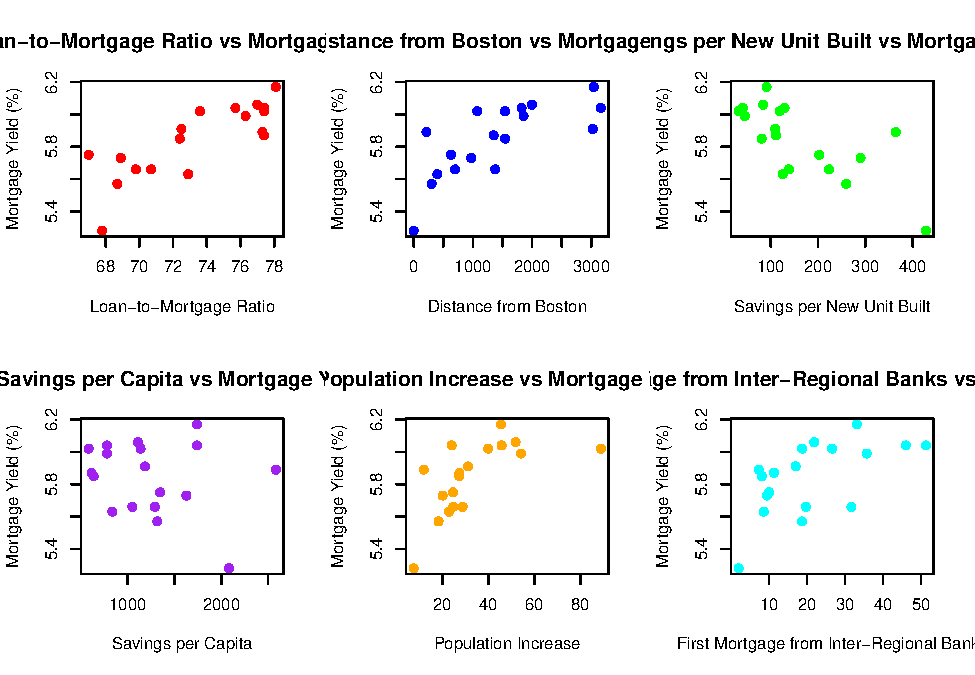
\includegraphics{report1_r1_files/figure-latex/unnamed-chunk-6-1.pdf}

\begin{Shaded}
\begin{Highlighting}[]
\CommentTok{\# Reset plotting parameters to default}
\FunctionTok{par}\NormalTok{(}\AttributeTok{mfrow =} \FunctionTok{c}\NormalTok{(}\DecValTok{1}\NormalTok{, }\DecValTok{1}\NormalTok{))}
\end{Highlighting}
\end{Shaded}

Let's take a closer look into the Association Matrix, regarding the
relationship between Mortgage Yield (\%) and the explanatory variables
(x-axis).\\
\textbf{1. Loan-to-Mortgage Ratio:} As this ratio increases, the
Mortgage Yield increases. This suggests a positive correlation, and that
higher loan-to-mortgage ratios (more borrowed money relative to the
property value) are associated with higher mortgage yields. This is
likely due to increased risk for lenders when down payments are low.\\
\textbf{2. Distance from Boston:} There is a positive correlation.
Boston represents a major financial center with surplus capital. Regions
further from Boston might have higher yields due to higher transfer
costs or credit shortages.\\
\textbf{3. Savings per New Unit Built :} There is a negative
correlation. This indicates that areas with more savings dedicated to
new construction have better access to local financing, resulting in
lower mortgage yields. It reflects regional credit demand and its
influence on yield determination.\\
\textbf{4. Savings per Capita:} The relationship is less clear but
appears to be a weak negative correlation. This suggesting that greater
local savings levels (credit supply) may reduce the need for external
financing. However, the impact is not as strong as the previous plots.\\
\textbf{5. Population Increase:} There is a positive correlation. High
population growth may imply higher demand for housing, increasing
mortgage yields due to heightened competition for available funds.
Reflects regional economic growth and housing demand.\\
\textbf{6. First Mortgage from Inter-Regional Banks:} No clear trend. It
seems like the reliance on external financing (measured by the
percentage of first mortgages from inter-regional banks) does not
significantly influence mortgage yields. The absence of a trend could
indicate that other factors, such as local market structures and
policies, play a more prominent role.\\
\strut \\
\textbf{To resume:}\\
- Loan-to-Mortgage Ratio (X1), Distance from Boston (X2), and Population
Increase (X5) are the most influential variables positively correlated
with Mortgage Yield.\\
- Savings per New Unit Built (X3) is the most influential negative
variable, indicating that local savings availability can effectively
reduce yields.\\
- The Savings per Capita (X4) and External Financing (X6) variables show
weak relationships with mortgage yields.\\
- These observations support the findings of Schaaf (1966) that distance
from financial centers, risk factors, and local demand for savings
contribute to yield variations.\\

\subsubsection{Correlation analysis}\label{correlation-analysis}

\begin{Shaded}
\begin{Highlighting}[]
\CommentTok{\# Correlation Matrix}
\CommentTok{\# Compute correlation matrix}
\NormalTok{cor\_matrix }\OtherTok{\textless{}{-}} \FunctionTok{round}\NormalTok{(}\FunctionTok{cor}\NormalTok{(df[,}\DecValTok{2}\SpecialCharTok{:}\DecValTok{8}\NormalTok{]), }\DecValTok{2}\NormalTok{)  }\CommentTok{\# Excluding \textquotesingle{}smsa\textquotesingle{}}
\FunctionTok{kable}\NormalTok{(cor\_matrix, }\AttributeTok{caption =} \StringTok{"Correlation Matrix"}\NormalTok{) }\SpecialCharTok{\%\textgreater{}\%} \FunctionTok{kable\_styling}\NormalTok{()}
\end{Highlighting}
\end{Shaded}

\begin{longtable}[t]{lrrrrrrr}
\caption{\label{tab:unnamed-chunk-7}Correlation Matrix}\\
\toprule
 & mortYld & X1 & X2 & X3 & X4 & X5 & X6\\
\midrule
mortYld & 1.00 & 0.81 & 0.74 & -0.72 & -0.22 & 0.65 & 0.59\\
X1 & 0.81 & 1.00 & 0.53 & -0.52 & -0.12 & 0.57 & 0.46\\
X2 & 0.74 & 0.53 & 1.00 & -0.64 & -0.14 & 0.44 & 0.60\\
X3 & -0.72 & -0.52 & -0.64 & 1.00 & 0.77 & -0.63 & -0.56\\
X4 & -0.22 & -0.12 & -0.14 & 0.77 & 1.00 & -0.40 & -0.23\\
\addlinespace
X5 & 0.65 & 0.57 & 0.44 & -0.63 & -0.40 & 1.00 & 0.39\\
X6 & 0.59 & 0.46 & 0.60 & -0.56 & -0.23 & 0.39 & 1.00\\
\bottomrule
\end{longtable}

\begin{Shaded}
\begin{Highlighting}[]
\FunctionTok{cor}\NormalTok{(}\FunctionTok{residuals}\NormalTok{(}\FunctionTok{lm}\NormalTok{(df}\SpecialCharTok{$}\NormalTok{X2 }\SpecialCharTok{\textasciitilde{}}\NormalTok{ df}\SpecialCharTok{$}\NormalTok{X3)), }\FunctionTok{residuals}\NormalTok{(}\FunctionTok{lm}\NormalTok{(df}\SpecialCharTok{$}\NormalTok{X6 }\SpecialCharTok{\textasciitilde{}}\NormalTok{ df}\SpecialCharTok{$}\NormalTok{X3)))}
\end{Highlighting}
\end{Shaded}

\begin{verbatim}
## [1] 0.3760938
\end{verbatim}

We see that X2 is only weakly positively correlated (r = 0.21) to X6
after controlling for X3; compare this to the much higher simple
correlation (r = 0.60). In other words, much of the apparent correlation
between X2 and X6 can be explained by their mutual positive correlation
with X3.

Numerical interpretation : LINEAR RELASHIONSHIPS

X3 (Savings per New Unit Built) and X4 (Savings per Capita) seem to be
strongly correlated (0.77). X2 (Distance from Boston) and X3 (Savings
per New Unit Built) have a high negative correlation (-0.64). X3
(Savings per New Unit Built) is also negatively correlated with X5
(Population Growth) at -0.63.

We can then think about removing one of the highly correlated
predictors, if multicollinearity affects the regression model.

numerical value of r : curve ? outliers? parallel lines?

\subsubsection{Graphical : Heatmap and Scatter
Plot}\label{graphical-heatmap-and-scatter-plot}

\begin{Shaded}
\begin{Highlighting}[]
\FunctionTok{library}\NormalTok{(ggplot2)}
\FunctionTok{library}\NormalTok{(reshape2)}
\end{Highlighting}
\end{Shaded}

\begin{verbatim}
## Warning: le package 'reshape2' a été compilé avec la version R 4.4.3
\end{verbatim}

\begin{verbatim}
## 
## Attachement du package : 'reshape2'
\end{verbatim}

\begin{verbatim}
## L'objet suivant est masqué depuis 'package:tidyr':
## 
##     smiths
\end{verbatim}

\begin{Shaded}
\begin{Highlighting}[]
\CommentTok{\# Convert correlation matrix to long format for heatmap}
\NormalTok{melted\_cor }\OtherTok{\textless{}{-}} \FunctionTok{melt}\NormalTok{(cor\_matrix)}

\CommentTok{\# Reverse the order of the y{-}axis (Var2) so that X1 appears at the top{-}left}
\FunctionTok{ggplot}\NormalTok{(}\AttributeTok{data =}\NormalTok{ melted\_cor, }\FunctionTok{aes}\NormalTok{(}\AttributeTok{x=}\NormalTok{Var1, }\AttributeTok{y=}\FunctionTok{factor}\NormalTok{(Var2, }\AttributeTok{levels=}\FunctionTok{rev}\NormalTok{(}\FunctionTok{unique}\NormalTok{(Var2))), }\AttributeTok{fill=}\NormalTok{value)) }\SpecialCharTok{+} 
  \FunctionTok{geom\_tile}\NormalTok{() }\SpecialCharTok{+}
  \FunctionTok{scale\_fill\_gradient2}\NormalTok{(}\AttributeTok{low=}\StringTok{"blue"}\NormalTok{, }\AttributeTok{high=}\StringTok{"red"}\NormalTok{, }\AttributeTok{mid=}\StringTok{"white"}\NormalTok{, }
                       \AttributeTok{midpoint=}\DecValTok{0}\NormalTok{, }\AttributeTok{limit=}\FunctionTok{c}\NormalTok{(}\SpecialCharTok{{-}}\DecValTok{1}\NormalTok{,}\DecValTok{1}\NormalTok{), }\AttributeTok{space=}\StringTok{"Lab"}\NormalTok{) }\SpecialCharTok{+}
  \FunctionTok{scale\_x\_discrete}\NormalTok{(}\AttributeTok{position =} \StringTok{"top"}\NormalTok{) }\SpecialCharTok{+}  \CommentTok{\# Move X{-}axis labels to top}
  \FunctionTok{theme\_minimal}\NormalTok{() }\SpecialCharTok{+}
  \FunctionTok{coord\_fixed}\NormalTok{() }\SpecialCharTok{+}
  \FunctionTok{theme}\NormalTok{(}\AttributeTok{axis.text.x =} \FunctionTok{element\_text}\NormalTok{(}\AttributeTok{angle =} \DecValTok{45}\NormalTok{, }\AttributeTok{hjust =} \DecValTok{0}\NormalTok{)) }\SpecialCharTok{+} \CommentTok{\# Rotate labels for readability}
  \FunctionTok{ggtitle}\NormalTok{(}\StringTok{"Correlation Heatmap"}\NormalTok{)}
\end{Highlighting}
\end{Shaded}

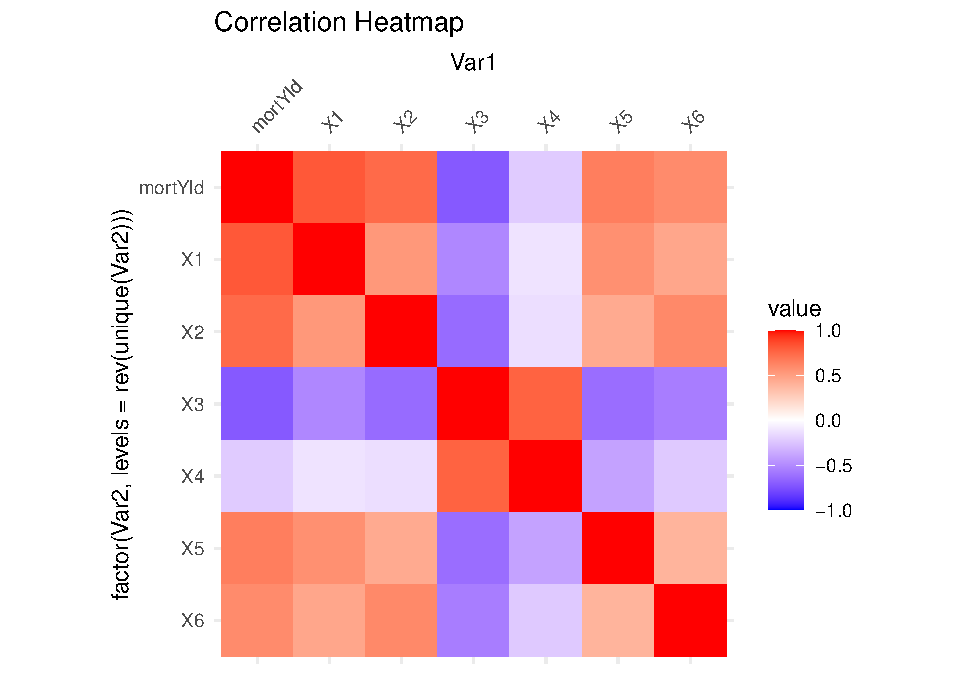
\includegraphics{report1_r1_files/figure-latex/unnamed-chunk-9-1.pdf}

\subsubsection{faire une dispersion matrix ? slide 28 cours
2}\label{faire-une-dispersion-matrix-slide-28-cours-2}

\begin{center}\rule{0.5\linewidth}{0.5pt}\end{center}

\section{Model Fitting}\label{model-fitting}

\subsection{Pairwise Simple
Regressions}\label{pairwise-simple-regressions}

\begin{Shaded}
\begin{Highlighting}[]
\CommentTok{\# Pairwise Simple Regressions}
\NormalTok{models\_simple }\OtherTok{\textless{}{-}} \FunctionTok{lapply}\NormalTok{(}\DecValTok{1}\SpecialCharTok{:}\DecValTok{6}\NormalTok{, }\ControlFlowTok{function}\NormalTok{(i) \{}
\NormalTok{  formula }\OtherTok{\textless{}{-}} \FunctionTok{as.formula}\NormalTok{(}\FunctionTok{paste}\NormalTok{(}\StringTok{"mortYld \textasciitilde{} X"}\NormalTok{, i, }\AttributeTok{sep =} \StringTok{""}\NormalTok{))}
  \FunctionTok{lm}\NormalTok{(formula, }\AttributeTok{data =}\NormalTok{ df)}
\NormalTok{\})}

\NormalTok{simple\_summaries }\OtherTok{\textless{}{-}} \FunctionTok{lapply}\NormalTok{(models\_simple, summary)}

\FunctionTok{data.frame}\NormalTok{(}
  \AttributeTok{Predictor =} \FunctionTok{paste0}\NormalTok{(}\StringTok{"X"}\NormalTok{, }\DecValTok{1}\SpecialCharTok{:}\DecValTok{6}\NormalTok{),}
  \AttributeTok{R\_squared =} \FunctionTok{sapply}\NormalTok{(simple\_summaries, }\ControlFlowTok{function}\NormalTok{(m) }\FunctionTok{round}\NormalTok{(m}\SpecialCharTok{$}\NormalTok{r.squared, }\DecValTok{3}\NormalTok{)),}
  \AttributeTok{p\_value =} \FunctionTok{sapply}\NormalTok{(simple\_summaries, }\ControlFlowTok{function}\NormalTok{(m) }\FunctionTok{round}\NormalTok{(}\FunctionTok{coef}\NormalTok{(m)[}\DecValTok{2}\NormalTok{,}\DecValTok{4}\NormalTok{], }\DecValTok{4}\NormalTok{))}
\NormalTok{) }\SpecialCharTok{\%\textgreater{}\%}
  \FunctionTok{kable}\NormalTok{(}\AttributeTok{caption =} \StringTok{"Simple Linear Regressions: R² and p{-}values"}\NormalTok{) }\SpecialCharTok{\%\textgreater{}\%}
  \FunctionTok{kable\_styling}\NormalTok{()}
\end{Highlighting}
\end{Shaded}

\begin{longtable}[t]{lrr}
\caption{\label{tab:unnamed-chunk-10}Simple Linear Regressions: R² and p-values}\\
\toprule
Predictor & R\_squared & p\_value\\
\midrule
X1 & 0.654 & 0.0000\\
X2 & 0.546 & 0.0005\\
X3 & 0.517 & 0.0008\\
X4 & 0.049 & 0.3763\\
X5 & 0.419 & 0.0037\\
\addlinespace
X6 & 0.346 & 0.0103\\
\bottomrule
\end{longtable}

\subsection{Null Model vs Full Model
Comparison}\label{null-model-vs-full-model-comparison}

\begin{Shaded}
\begin{Highlighting}[]
\CommentTok{\# Null Model vs Full Model Comparison}
\NormalTok{null\_model }\OtherTok{\textless{}{-}} \FunctionTok{lm}\NormalTok{(mortYld }\SpecialCharTok{\textasciitilde{}} \DecValTok{1}\NormalTok{, }\AttributeTok{data =}\NormalTok{ df)}
\NormalTok{full\_model }\OtherTok{\textless{}{-}} \FunctionTok{lm}\NormalTok{(mortYld }\SpecialCharTok{\textasciitilde{}}\NormalTok{ X1 }\SpecialCharTok{+}\NormalTok{ X2 }\SpecialCharTok{+}\NormalTok{ X3 }\SpecialCharTok{+}\NormalTok{ X4 }\SpecialCharTok{+}\NormalTok{ X5 }\SpecialCharTok{+}\NormalTok{ X6, }\AttributeTok{data =}\NormalTok{ df)}

\FunctionTok{anova}\NormalTok{(null\_model, full\_model)}
\end{Highlighting}
\end{Shaded}

\begin{verbatim}
## Analysis of Variance Table
## 
## Model 1: mortYld ~ 1
## Model 2: mortYld ~ X1 + X2 + X3 + X4 + X5 + X6
##   Res.Df     RSS Df Sum of Sq      F    Pr(>F)    
## 1     17 0.84858                                  
## 2     11 0.10980  6   0.73877 12.335 0.0002523 ***
## ---
## Signif. codes:  0 '***' 0.001 '**' 0.01 '*' 0.05 '.' 0.1 ' ' 1
\end{verbatim}

Here we can see that the Null model don't fit the data. We really should
the variables.

\begin{Shaded}
\begin{Highlighting}[]
\CommentTok{\# Fit linear regression model}
\NormalTok{model }\OtherTok{\textless{}{-}} \FunctionTok{lm}\NormalTok{(mortYld }\SpecialCharTok{\textasciitilde{}}\NormalTok{ X1 }\SpecialCharTok{+}\NormalTok{ X2 }\SpecialCharTok{+}\NormalTok{ X3 }\SpecialCharTok{+}\NormalTok{ X4 }\SpecialCharTok{+}\NormalTok{ X5 }\SpecialCharTok{+}\NormalTok{ X6, }\AttributeTok{data =}\NormalTok{ df)}

\CommentTok{\# Model summary}
\FunctionTok{summary}\NormalTok{(model)}
\end{Highlighting}
\end{Shaded}

\begin{verbatim}
## 
## Call:
## lm(formula = mortYld ~ X1 + X2 + X3 + X4 + X5 + X6, data = df)
## 
## Residuals:
##       Min        1Q    Median        3Q       Max 
## -0.145030 -0.017814  0.001474  0.034316  0.134565 
## 
## Coefficients:
##               Estimate Std. Error t value Pr(>|t|)    
## (Intercept)  4.285e+00  6.682e-01   6.413 4.99e-05 ***
## X1           2.033e-02  9.308e-03   2.184   0.0515 .  
## X2           1.359e-05  4.692e-05   0.290   0.7775    
## X3          -1.584e-03  7.532e-04  -2.103   0.0593 .  
## X4           2.017e-04  1.124e-04   1.794   0.1002    
## X5           1.283e-03  1.765e-03   0.727   0.4826    
## X6           2.357e-04  2.302e-03   0.102   0.9203    
## ---
## Signif. codes:  0 '***' 0.001 '**' 0.01 '*' 0.05 '.' 0.1 ' ' 1
## 
## Residual standard error: 0.09991 on 11 degrees of freedom
## Multiple R-squared:  0.8706, Adjusted R-squared:    0.8 
## F-statistic: 12.33 on 6 and 11 DF,  p-value: 0.0002523
\end{verbatim}

\subsection{Make stepwise regression to select the best
model}\label{make-stepwise-regression-to-select-the-best-model}

By removing some of the variables

\begin{Shaded}
\begin{Highlighting}[]
\CommentTok{\# Stepwise regression (both directions)}
\NormalTok{step\_model }\OtherTok{\textless{}{-}} \FunctionTok{stepAIC}\NormalTok{(model, }\AttributeTok{direction =} \StringTok{"both"}\NormalTok{)}
\end{Highlighting}
\end{Shaded}

\begin{verbatim}
## Start:  AIC=-77.79
## mortYld ~ X1 + X2 + X3 + X4 + X5 + X6
## 
##        Df Sum of Sq     RSS     AIC
## - X6    1  0.000105 0.10991 -79.773
## - X2    1  0.000837 0.11064 -79.653
## - X5    1  0.005271 0.11507 -78.946
## <none>              0.10980 -77.790
## - X4    1  0.032141 0.14194 -75.168
## - X3    1  0.044144 0.15395 -73.707
## - X1    1  0.047593 0.15740 -73.308
## 
## Step:  AIC=-79.77
## mortYld ~ X1 + X2 + X3 + X4 + X5
## 
##        Df Sum of Sq     RSS     AIC
## - X2    1  0.000971 0.11088 -81.614
## - X5    1  0.005259 0.11517 -80.931
## <none>              0.10991 -79.773
## + X6    1  0.000105 0.10980 -77.790
## - X4    1  0.033056 0.14297 -77.040
## - X3    1  0.046942 0.15685 -75.371
## - X1    1  0.048227 0.15813 -75.224
## 
## Step:  AIC=-81.61
## mortYld ~ X1 + X3 + X4 + X5
## 
##        Df Sum of Sq     RSS     AIC
## - X5    1  0.005047 0.11593 -82.813
## <none>              0.11088 -81.614
## + X2    1  0.000971 0.10991 -79.773
## + X6    1  0.000238 0.11064 -79.653
## - X1    1  0.047325 0.15820 -77.216
## - X4    1  0.076985 0.18786 -74.123
## - X3    1  0.139427 0.25031 -68.958
## 
## Step:  AIC=-82.81
## mortYld ~ X1 + X3 + X4
## 
##        Df Sum of Sq     RSS     AIC
## <none>              0.11593 -82.813
## + X5    1  0.005047 0.11088 -81.614
## + X2    1  0.000759 0.11517 -80.931
## + X6    1  0.000202 0.11572 -80.845
## - X1    1  0.065583 0.18151 -76.743
## - X4    1  0.075826 0.19175 -75.755
## - X3    1  0.164703 0.28063 -68.900
\end{verbatim}

\begin{Shaded}
\begin{Highlighting}[]
\FunctionTok{summary}\NormalTok{(step\_model)}
\end{Highlighting}
\end{Shaded}

\begin{verbatim}
## 
## Call:
## lm(formula = mortYld ~ X1 + X3 + X4, data = df)
## 
## Residuals:
##       Min        1Q    Median        3Q       Max 
## -0.172291 -0.018862  0.006091  0.040552  0.145956 
## 
## Coefficients:
##               Estimate Std. Error t value Pr(>|t|)    
## (Intercept)  4.223e+00  5.814e-01   7.263 4.14e-06 ***
## X1           2.229e-02  7.922e-03   2.814 0.013787 *  
## X3          -1.863e-03  4.178e-04  -4.460 0.000539 ***
## X4           2.249e-04  7.433e-05   3.026 0.009070 ** 
## ---
## Signif. codes:  0 '***' 0.001 '**' 0.01 '*' 0.05 '.' 0.1 ' ' 1
## 
## Residual standard error: 0.091 on 14 degrees of freedom
## Multiple R-squared:  0.8634, Adjusted R-squared:  0.8341 
## F-statistic: 29.49 on 3 and 14 DF,  p-value: 2.618e-06
\end{verbatim}

The stepwise regression process identified X1, X3, and X4 as the most
significant predictors of mortality yield, leading to the final model:\\
mortYld = 4.223 + 0.02229.X1 − 0.001863.X3 + 0.0002249.X4\\
Now we will test a model with 3-way interactions.

\begin{Shaded}
\begin{Highlighting}[]
\CommentTok{\#model with interactions}
\NormalTok{interaction\_model }\OtherTok{\textless{}{-}} \FunctionTok{lm}\NormalTok{(mortYld }\SpecialCharTok{\textasciitilde{}}\NormalTok{ X1 }\SpecialCharTok{*}\NormalTok{ X3 }\SpecialCharTok{*}\NormalTok{ X4, }\AttributeTok{data =}\NormalTok{ df)}

\CommentTok{\# Summary of the model}
\FunctionTok{summary}\NormalTok{(interaction\_model)}
\end{Highlighting}
\end{Shaded}

\begin{verbatim}
## 
## Call:
## lm(formula = mortYld ~ X1 * X3 * X4, data = df)
## 
## Residuals:
##       Min        1Q    Median        3Q       Max 
## -0.152588 -0.048599  0.008586  0.043241  0.128805 
## 
## Coefficients:
##               Estimate Std. Error t value Pr(>|t|)
## (Intercept)  1.272e+00  3.455e+00   0.368    0.720
## X1           6.233e-02  4.623e-02   1.348    0.207
## X3           2.785e-02  2.154e-02   1.293    0.225
## X4           1.421e-03  2.852e-03   0.498    0.629
## X1:X3       -4.049e-04  2.959e-04  -1.368    0.201
## X1:X4       -1.638e-05  3.777e-05  -0.434    0.674
## X3:X4       -1.412e-05  9.817e-06  -1.438    0.181
## X1:X3:X4     1.917e-07  1.336e-07   1.434    0.182
## 
## Residual standard error: 0.09572 on 10 degrees of freedom
## Multiple R-squared:  0.892,  Adjusted R-squared:  0.8165 
## F-statistic:  11.8 on 7 and 10 DF,  p-value: 0.000408
\end{verbatim}

The model complexity increased, but there was no significant improvement
in performance.\\
Let's try a model with only 2-way interactions, and use a AIC step-wise
selection to select only relevant interactions

\begin{Shaded}
\begin{Highlighting}[]
\NormalTok{reduced\_interaction\_model }\OtherTok{\textless{}{-}} \FunctionTok{lm}\NormalTok{(mortYld }\SpecialCharTok{\textasciitilde{}}\NormalTok{ X1 }\SpecialCharTok{+}\NormalTok{ X3 }\SpecialCharTok{+}\NormalTok{ X4 }\SpecialCharTok{+}\NormalTok{ X1}\SpecialCharTok{:}\NormalTok{X3 }\SpecialCharTok{+}\NormalTok{ X1}\SpecialCharTok{:}\NormalTok{X4 }\SpecialCharTok{+}\NormalTok{ X3}\SpecialCharTok{:}\NormalTok{X4, }\AttributeTok{data =}\NormalTok{ df)}
\FunctionTok{summary}\NormalTok{(reduced\_interaction\_model)}
\end{Highlighting}
\end{Shaded}

\begin{verbatim}
## 
## Call:
## lm(formula = mortYld ~ X1 + X3 + X4 + X1:X3 + X1:X4 + X3:X4, 
##     data = df)
## 
## Residuals:
##       Min        1Q    Median        3Q       Max 
## -0.187649 -0.015613  0.007221  0.030851  0.155167 
## 
## Coefficients:
##               Estimate Std. Error t value Pr(>|t|)  
## (Intercept)  5.371e+00  2.033e+00   2.642   0.0229 *
## X1           6.912e-03  2.657e-02   0.260   0.7996  
## X3          -1.040e-04  9.611e-03  -0.011   0.9916  
## X4          -9.096e-04  2.454e-03  -0.371   0.7180  
## X1:X3       -2.091e-05  1.322e-04  -0.158   0.8772  
## X1:X4        1.497e-05  3.225e-05   0.464   0.6516  
## X3:X4       -4.751e-08  4.540e-07  -0.105   0.9185  
## ---
## Signif. codes:  0 '***' 0.001 '**' 0.01 '*' 0.05 '.' 0.1 ' ' 1
## 
## Residual standard error: 0.1002 on 11 degrees of freedom
## Multiple R-squared:  0.8698, Adjusted R-squared:  0.7988 
## F-statistic: 12.25 on 6 and 11 DF,  p-value: 0.0002604
\end{verbatim}

\begin{Shaded}
\begin{Highlighting}[]
\NormalTok{step\_interaction\_model }\OtherTok{\textless{}{-}} \FunctionTok{stepAIC}\NormalTok{(}\FunctionTok{lm}\NormalTok{(mortYld }\SpecialCharTok{\textasciitilde{}}\NormalTok{ X1 }\SpecialCharTok{*}\NormalTok{ X3 }\SpecialCharTok{*}\NormalTok{ X4, }\AttributeTok{data =}\NormalTok{ df), }\AttributeTok{direction =} \StringTok{"both"}\NormalTok{)}
\end{Highlighting}
\end{Shaded}

\begin{verbatim}
## Start:  AIC=-79.05
## mortYld ~ X1 * X3 * X4
## 
##            Df Sum of Sq      RSS     AIC
## <none>                  0.091614 -79.050
## - X1:X3:X4  1  0.018851 0.110465 -77.682
\end{verbatim}

\begin{Shaded}
\begin{Highlighting}[]
\FunctionTok{summary}\NormalTok{(step\_interaction\_model)}
\end{Highlighting}
\end{Shaded}

\begin{verbatim}
## 
## Call:
## lm(formula = mortYld ~ X1 * X3 * X4, data = df)
## 
## Residuals:
##       Min        1Q    Median        3Q       Max 
## -0.152588 -0.048599  0.008586  0.043241  0.128805 
## 
## Coefficients:
##               Estimate Std. Error t value Pr(>|t|)
## (Intercept)  1.272e+00  3.455e+00   0.368    0.720
## X1           6.233e-02  4.623e-02   1.348    0.207
## X3           2.785e-02  2.154e-02   1.293    0.225
## X4           1.421e-03  2.852e-03   0.498    0.629
## X1:X3       -4.049e-04  2.959e-04  -1.368    0.201
## X1:X4       -1.638e-05  3.777e-05  -0.434    0.674
## X3:X4       -1.412e-05  9.817e-06  -1.438    0.181
## X1:X3:X4     1.917e-07  1.336e-07   1.434    0.182
## 
## Residual standard error: 0.09572 on 10 degrees of freedom
## Multiple R-squared:  0.892,  Adjusted R-squared:  0.8165 
## F-statistic:  11.8 on 7 and 10 DF,  p-value: 0.000408
\end{verbatim}

This model is worse then with all 3-way interactions.

\subsection{Model Comparison}\label{model-comparison}

\begin{Shaded}
\begin{Highlighting}[]
\CommentTok{\# Compare model performances}
\NormalTok{adj\_r2\_compare }\OtherTok{\textless{}{-}} \FunctionTok{data.frame}\NormalTok{(}
  \AttributeTok{Model =} \FunctionTok{c}\NormalTok{(}\StringTok{"Full Model"}\NormalTok{, }\StringTok{"Stepwise Model"}\NormalTok{, }\StringTok{"2{-}Way Interaction Model"}\NormalTok{),}
  \AttributeTok{Adj\_R2 =} \FunctionTok{c}\NormalTok{(}
    \FunctionTok{summary}\NormalTok{(full\_model)}\SpecialCharTok{$}\NormalTok{adj.r.squared,}
    \FunctionTok{summary}\NormalTok{(step\_model)}\SpecialCharTok{$}\NormalTok{adj.r.squared,}
    \FunctionTok{summary}\NormalTok{(reduced\_interaction\_model)}\SpecialCharTok{$}\NormalTok{adj.r.squared}
\NormalTok{  )}
\NormalTok{)}

\FunctionTok{kable}\NormalTok{(adj\_r2\_compare, }\AttributeTok{caption =} \StringTok{"Adjusted R² for Different Models"}\NormalTok{) }\SpecialCharTok{\%\textgreater{}\%} \FunctionTok{kable\_styling}\NormalTok{()}
\end{Highlighting}
\end{Shaded}

\begin{longtable}[t]{lr}
\caption{\label{tab:unnamed-chunk-16}Adjusted R² for Different Models}\\
\toprule
Model & Adj\_R2\\
\midrule
Full Model & 0.8000222\\
Stepwise Model & 0.8341136\\
2-Way Interaction Model & 0.7988172\\
\bottomrule
\end{longtable}

\begin{Shaded}
\begin{Highlighting}[]
\CommentTok{\# Compare AIC}
\NormalTok{aic\_compare }\OtherTok{\textless{}{-}} \FunctionTok{AIC}\NormalTok{(full\_model, step\_model, reduced\_interaction\_model)}
\FunctionTok{kable}\NormalTok{(aic\_compare, }\AttributeTok{caption =} \StringTok{"AIC for Different Models"}\NormalTok{) }\SpecialCharTok{\%\textgreater{}\%} \FunctionTok{kable\_styling}\NormalTok{()}
\end{Highlighting}
\end{Shaded}

\begin{longtable}[t]{lrr}
\caption{\label{tab:unnamed-chunk-16}AIC for Different Models}\\
\toprule
 & df & AIC\\
\midrule
full\_model & 8 & -24.70799\\
step\_model & 5 & -29.73133\\
reduced\_interaction\_model & 8 & -24.59986\\
\bottomrule
\end{longtable}

\begin{Shaded}
\begin{Highlighting}[]
\CommentTok{\# Compare with ANOVA}
\FunctionTok{anova}\NormalTok{(full\_model, step\_model, reduced\_interaction\_model)}
\end{Highlighting}
\end{Shaded}

\begin{verbatim}
## Analysis of Variance Table
## 
## Model 1: mortYld ~ X1 + X2 + X3 + X4 + X5 + X6
## Model 2: mortYld ~ X1 + X3 + X4
## Model 3: mortYld ~ X1 + X3 + X4 + X1:X3 + X1:X4 + X3:X4
##   Res.Df     RSS Df  Sum of Sq      F Pr(>F)
## 1     11 0.10980                            
## 2     14 0.11593 -3 -0.0061224 0.2044 0.8912
## 3     11 0.11046  3  0.0054608 0.1824 0.9062
\end{verbatim}

\begin{center}\rule{0.5\linewidth}{0.5pt}\end{center}

\section{Model assumptions and
Diagnostics}\label{model-assumptions-and-diagnostics}

\subsection{Multicolinearity Check using
VIF}\label{multicolinearity-check-using-vif}

\begin{description}
\item[a VIF \textgreater{} 5 indicates possible multicollinearity that
can be problematic]
we are not able to identify the variables associated with this
collinearity but we will have to do it next.
\end{description}

\begin{Shaded}
\begin{Highlighting}[]
\CommentTok{\# Compute Variance Inflation Factor (VIF)}
\NormalTok{vif\_values }\OtherTok{\textless{}{-}} \FunctionTok{vif}\NormalTok{(model)}
\FunctionTok{kable}\NormalTok{(}\FunctionTok{as.data.frame}\NormalTok{(vif\_values), }\AttributeTok{caption =} \StringTok{"Variance Inflation Factors (VIF)"}\NormalTok{) }\SpecialCharTok{\%\textgreater{}\%} \FunctionTok{kable\_styling}\NormalTok{()}
\end{Highlighting}
\end{Shaded}

\begin{longtable}[t]{lr}
\caption{\label{tab:unnamed-chunk-17}Variance Inflation Factors (VIF)}\\
\toprule
 & vif\_values\\
\midrule
X1 & 2.161053\\
X2 & 3.564189\\
X3 & 12.267210\\
X4 & 6.349640\\
X5 & 1.927806\\
\addlinespace
X6 & 1.750673\\
\bottomrule
\end{longtable}

\subsection{Residuals Analysis}\label{residuals-analysis}

Random scatter indicates good assumption of homeoscedasticity. If we can
distinguish a clear pattern, then we have potential heteroscedasticity
issue.

\begin{Shaded}
\begin{Highlighting}[]
\CommentTok{\# Residuals vs Fitted Plot}
\FunctionTok{ggplot}\NormalTok{(}\FunctionTok{data.frame}\NormalTok{(}\AttributeTok{fitted =} \FunctionTok{fitted}\NormalTok{(model), }\AttributeTok{residuals =} \FunctionTok{resid}\NormalTok{(model)), }\FunctionTok{aes}\NormalTok{(}\AttributeTok{x =}\NormalTok{ fitted, }\AttributeTok{y =}\NormalTok{ residuals)) }\SpecialCharTok{+}
  \FunctionTok{geom\_point}\NormalTok{(}\AttributeTok{alpha =} \FloatTok{0.5}\NormalTok{) }\SpecialCharTok{+}
  \FunctionTok{geom\_hline}\NormalTok{(}\AttributeTok{yintercept =} \DecValTok{0}\NormalTok{, }\AttributeTok{linetype =} \StringTok{"dashed"}\NormalTok{) }\SpecialCharTok{+}
  \FunctionTok{labs}\NormalTok{(}\AttributeTok{title =} \StringTok{"Residuals vs Fitted Plot"}\NormalTok{, }\AttributeTok{x =} \StringTok{"Fitted Values"}\NormalTok{, }\AttributeTok{y =} \StringTok{"Residuals"}\NormalTok{)}
\end{Highlighting}
\end{Shaded}

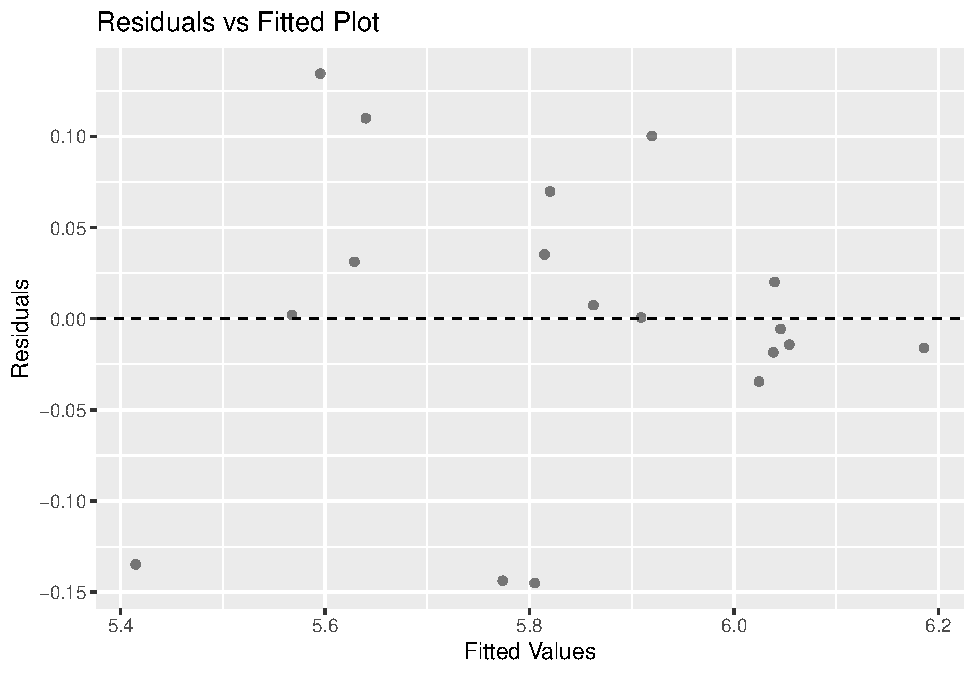
\includegraphics{report1_r1_files/figure-latex/unnamed-chunk-18-1.pdf}

\subsection{Normality Check}\label{normality-check}

If points lie on 45 degrees line, it means the residuals are normally
distributed. If we can see a curved pattern, then the normality
assumption is violated

\begin{Shaded}
\begin{Highlighting}[]
\CommentTok{\# QQ{-}Plot of Residuals}
\NormalTok{residuals }\OtherTok{\textless{}{-}} \FunctionTok{resid}\NormalTok{(model)  }\CommentTok{\# Extract residuals}

\CommentTok{\# Set up a square plotting area}
\FunctionTok{par}\NormalTok{(}\AttributeTok{pty =} \StringTok{"s"}\NormalTok{)  }

\CommentTok{\# Generate the Q{-}Q plot}
\FunctionTok{qqnorm}\NormalTok{(residuals, }\AttributeTok{main =} \StringTok{"Q{-}Q Plot of Residuals"}\NormalTok{) }\CommentTok{\#Normal Q{-}Q Plot}
\FunctionTok{qqline}\NormalTok{(residuals, }\AttributeTok{col =} \StringTok{"red"}\NormalTok{)}
\end{Highlighting}
\end{Shaded}

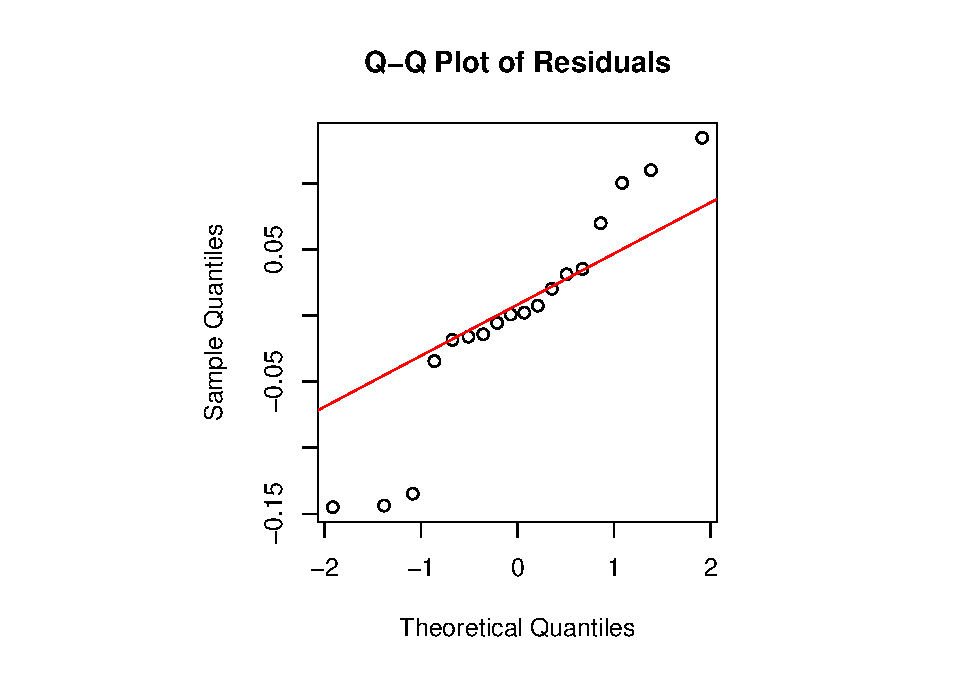
\includegraphics{report1_r1_files/figure-latex/unnamed-chunk-19-1.pdf}

\begin{Shaded}
\begin{Highlighting}[]
\CommentTok{\# Reset plotting parameters (optional)}
\FunctionTok{par}\NormalTok{(}\AttributeTok{pty =} \StringTok{"m"}\NormalTok{)  }
\end{Highlighting}
\end{Shaded}

\begin{center}\rule{0.5\linewidth}{0.5pt}\end{center}

\section{Final estimated Model}\label{final-estimated-model}

\begin{Shaded}
\begin{Highlighting}[]
\NormalTok{coeffs }\OtherTok{\textless{}{-}} \FunctionTok{round}\NormalTok{(}\FunctionTok{coef}\NormalTok{(model), }\DecValTok{2}\NormalTok{)}
\FunctionTok{kable}\NormalTok{(}\FunctionTok{as.data.frame}\NormalTok{(coeffs), }\AttributeTok{caption =} \StringTok{"Final Model Coefficients"}\NormalTok{) }\SpecialCharTok{\%\textgreater{}\%} \FunctionTok{kable\_styling}\NormalTok{()}
\end{Highlighting}
\end{Shaded}

\begin{longtable}[t]{lr}
\caption{\label{tab:unnamed-chunk-20}Final Model Coefficients}\\
\toprule
 & coeffs\\
\midrule
(Intercept) & 4.29\\
X1 & 0.02\\
X2 & 0.00\\
X3 & 0.00\\
X4 & 0.00\\
\addlinespace
X5 & 0.00\\
X6 & 0.00\\
\bottomrule
\end{longtable}

\begin{center}\rule{0.5\linewidth}{0.5pt}\end{center}

\section{Conclusions}\label{conclusions}

\begin{verbatim}
•   The analysis showed that [mention significant predictors] have a strong relationship with mortgage yield.
•   The assumptions of linear regression were [state if met or violated].
•   The model provides [good/poor] predictive accuracy based on [R² and residual analysis].
•   Future improvements could involve [mention possible improvements like transformations, additional predictors, etc.].
\end{verbatim}

\end{document}
